% SPDX-License-Identifier: CC-BY-SA-4.0
% Author: Matthieu Perrin
% Part: 
% Section: 
% Sub-section: 
% Frame: 

\begingroup

\begin{frame}[fragile]{Cohérence de cache}
  \begin{block}{Architectures UMA (Uniform Memory Access)}
    \begin{center}
      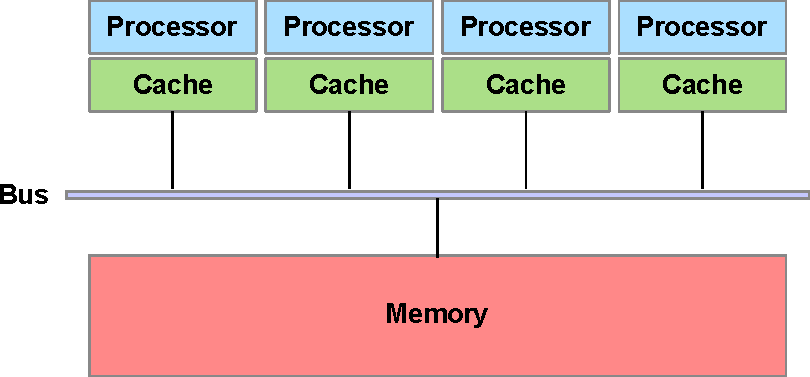
\includegraphics[height=1.8cm]{uma}
    \end{center}
  \end{block}
  \begin{exampleblock}{Mot-clé \lstinline{volatile int x;} (depuis Java 5)}
    \begin{itemize}
    \item Tout le cache est invalidé \structure{avant chaque lecture}  de $x$
    \item Tout le cache est invalidé \structure{après chaque écriture} de $x$
    \item Le cache n'est pas invalidé \structure{pendant} une lecture ou écriture de $x$ \footnote{
      \href{https://docs.oracle.com/javase/specs/jls/se7/html/jls-17.html\#jls-17.7}{(§17.7)}
      Implementations of the Java Virtual Machine are \alert{encouraged} to avoid splitting 64-bit values where possible.
      Programmers are \alert{encouraged} to declare shared 64-bit values as volatile or synchronize their programs correctly to avoid possible complications.
      }
    \end{itemize}
  \end{exampleblock}
  \begin{alertblock}{Attention}
    \begin{itemize}
    \item Une invalidation de cache est très inefficace !
    \end{itemize}
  \end{alertblock}

\end{frame}

\endgroup
\endinput
